\chapter{Geometría}
%% texto a la izquierda y figura a la derecha: \geolado[fracción del ancho para la figura]{figura}{texto}
\newcommand{\geolado}[3][0.38]{\par\smallskip\noindent
  \begin{minipage}[c]{\dimexpr\linewidth-#1\linewidth-14pt\relax}\setlength{\parskip}{4pt}#3\end{minipage}\hspace{14pt}%
  \begin{minipage}[c]{#1\linewidth}\centering\includegraphics[width=\linewidth]{#2}\end{minipage}\par\smallskip}

%% =====================================================================
\section{Teorema de Pitágoras}
\subsection{El triángulo rectángulo y el teorema}
\geolado[0.27]{geo_pit_cuadrados}{Un \textbf{triángulo rectángulo} tiene un ángulo de 90°, que se marca con un cuadradito. Los dos lados que forman ese ángulo son los \textbf{catetos}; el lado que queda al frente es la \textbf{hipotenusa}, y siempre es el más largo.

En la figura, $3^2 + 4^2 = 9 + 16 = 25 = 5^2$: los cuadrados de los catetos juntos tienen la misma área que el cuadrado de la hipotenusa.}
\begin{clave}[Teorema de Pitágoras] Si los catetos miden $a$ y $b$ y la hipotenusa mide $c$, entonces \quad $a^2 + b^2 = c^2$.\end{clave}
\begin{ojo}[Solo para triángulos rectángulos] Si el triángulo no tiene un ángulo de 90°, el teorema no se cumple. Y la hipotenusa va sola en un lado de la igualdad.\end{ojo}

\subsection{Calcular la hipotenusa o un cateto}
\begin{clave}[Regla rápida] Falta la hipotenusa: \textbf{suma} los cuadrados, $c = \sqrt{a^2 + b^2}$. Falta un cateto: \textbf{resta} los cuadrados, al más grande el más chico, $a = \sqrt{c^2 - b^2}$.\end{clave}
\begin{ejemplo} Catetos de 6 cm y 8 cm: $c^2 = 36 + 64 = 100$, así que $c = \sqrt{100} = 10$ cm. Una escalera de 5 m apoyada en un muro, con el pie a 3 m de él, es la hipotenusa: $h^2 = 25 - 9 = 16$ y llega a $h = 4$ m de altura.\end{ejemplo}
\begin{ojo}[La raíz no se reparte] $\sqrt{36 + 64}$ no es $6 + 8 = 14$: primero se suma y después se saca la raíz, $\sqrt{100} = 10$. Además, $c^2 = 100$ todavía no es la respuesta. Si un cateto te sale más largo que la hipotenusa, sumaste cuando había que restar.\end{ojo}
\gatotip[\gatogris]{Antes de hacer cuentas, marca la hipotenusa: es el lado al frente del cuadradito. Escaleras, rampas, tensores y cuerdas inclinadas casi siempre lo son.}

\subsection{Tríos pitagóricos y el recíproco}
Un \textbf{trío pitagórico} son tres enteros que cumplen $a^2 + b^2 = c^2$. Reconocerlos ahorra cuentas, y al multiplicarlos por un mismo número siguen siendo tríos: $6, 8, 10$ es el doble de $3, 4, 5$, y $0{,}7;\ 2{,}4;\ 2{,}5$ es $7, 24, 25$ dividido por 10.
\begin{center}\small
\begin{tabular}{cccccc}\toprule
$3, 4, 5$ & $5, 12, 13$ & $8, 15, 17$ & $7, 24, 25$ & $12, 35, 37$ & $9, 40, 41$\\\bottomrule
\end{tabular}\end{center}
\begin{clave}[Recíproco del teorema] Si el cuadrado del lado mayor es igual a la suma de los cuadrados de los otros dos, el triángulo es rectángulo, y el ángulo recto está al frente del lado mayor.\end{clave}
\begin{ejemplo} Lados 9, 12 y 15: $81 + 144 = 225 = 15^2$ \checkmark, es rectángulo. Lados 4, 5 y 6: $16 + 25 = 41$, pero $6^2 = 36$: no lo es.\end{ejemplo}

\subsection{Diagonales de rectángulos y de cajas}
\geolado[0.42]{geo_pit_diagonales}{La diagonal parte un rectángulo en dos triángulos rectángulos: los lados son los catetos y la diagonal es la hipotenusa. En un cuadrado de lado $\ell$, $d^2 = 2\ell^2$ y $d = \ell\sqrt{2}$.

En una caja de aristas $a$, $b$ y $c$, la diagonal interior cumple \[D^2 = a^2 + b^2 + c^2,\] que sale de aplicar Pitágoras dos veces: primero en el piso y después con la altura.}
\begin{ejemplo} Caja de 2, 3 y 6 cm: $D^2 = 4 + 9 + 36 = 49$, así que $D = 7$ cm. Una pantalla con razón alto\,:\,ancho $= 9 : 16$ tiene alto $9x$ y ancho $16x$, con $x$ el factor de proporcionalidad, y su diagonal cumple $(9x)^2 + (16x)^2 = d^2$.\end{ejemplo}

\subsection{Distancia entre dos puntos del plano}
\geolado[0.33]{geo_pit_distancia}{Para medir la distancia entre $A(4, 2)$ y $B(10, 10)$ se arma un triángulo rectángulo con un cateto horizontal, $10 - 4 = 6$, y uno vertical, $10 - 2 = 8$. Entonces $d = \sqrt{36 + 64} = 10$.}
\begin{clave}[Distancia entre puntos] Entre $(x_1, y_1)$ y $(x_2, y_2)$: \quad $d = \sqrt{(x_2 - x_1)^2 + (y_2 - y_1)^2}$.\end{clave}
\begin{ojo}[Ojo con los negativos] Entre $(-2, 1)$ y $(4, 9)$ el cateto horizontal es $4 - (-2) = 6$, no $2$. Como se eleva al cuadrado, da lo mismo restar en un orden o en el otro.\end{ojo}
\gatotip[\gatoatigrado]{Busca triángulos escondidos: la altura de un triángulo isósceles cae justo al medio de la base, las diagonales de un rombo se cortan por la mitad en ángulo recto y en un trapecio rectángulo el cateto vertical es la diferencia de los lados paralelos.}

\begin{elejemplo}{PAES Invierno 2026, adaptada}
\geolado[0.3]{geo_pit_repisa}{Una persona debe confeccionar una repisa con dos tensores, tal como se representa en la imagen. Cada tensor une el borde superior del panel vertical, de 200 cm de alto, con el borde exterior de la tabla horizontal, de 150 cm de ancho.

Si la persona quiere calcular la medida que debe tener cada uno de los tensores, en centímetros, ¿cuál de las siguientes expresiones debe utilizar?}
\alts{$\sqrt{200^2 - 150^2}$}{$200^2 - 150^2$}{$\sqrt{200^2 + 150^2}$}{$200^2 + 150^2$}
\solucion{El panel vertical (200 cm) y la tabla horizontal (150 cm) forman un ángulo recto, y el tensor une sus extremos: está al frente del ángulo recto, así que es la \textbf{hipotenusa}. Si mide $t$, entonces $t^2 = 200^2 + 150^2$ y, sacando raíz, $t = \sqrt{200^2 + 150^2}$.

\textit{Comprobación}: $\sqrt{40.000 + 22.500} = \sqrt{62.500} = 250$ cm, más largo que 200 y que 150, como debe ser una hipotenusa (es el trío 3, 4, 5 multiplicado por 50) \checkmark.

\textit{¿Por qué no las otras?} $\sqrt{200^2 - 150^2}$ resta, como si faltara un cateto: daría unos 132 cm, menos que el panel. $200^2 - 150^2$ y $200^2 + 150^2$ olvidan la raíz: dan el cuadrado del largo, no el largo.}{C}
\end{elejemplo}
\motivacion{Pitágoras lleva más de dos mil años ayudando a estudiantes, y hoy te ayudó a ti. Tres lados, un teorema, cero miedo.}

%% =====================================================================
\section{Perímetro y área de triángulos, paralelogramos y trapecios}
\subsection{Perímetro y área: no son lo mismo}
El \textbf{perímetro} es el largo del borde: la suma de todos los lados, en unidades de largo (cm, m, km). El \textbf{área} mide la superficie de adentro: cuántos cuadraditos de $1 \times 1$ caben, en unidades cuadradas (cm$^2$, m$^2$).
\begin{ejemplo} Rectángulo de 6 cm por 4 cm: perímetro $2(6 + 4) = 20$ cm y área $6 \cdot 4 = 24$ cm$^2$. Cuadrado de lado 5 cm: perímetro $4 \cdot 5 = 20$ cm y área $5^2 = 25$ cm$^2$.\end{ejemplo}
\begin{ojo}[Cuidado con las unidades] El perímetro va en cm y el área en cm$^2$. Antes de calcular, pasa todo a la misma unidad: no multipliques metros por centímetros.\end{ojo}

\subsection{Área del triángulo: la altura correcta}
\geolado[0.45]{geo_ar_alturas}{Todo triángulo es la mitad de un rectángulo (o de un paralelogramo) con su misma base y su misma altura.

La \textbf{altura} es el segmento \textbf{perpendicular} a la base que llega al vértice opuesto; no es un lado inclinado.}
\begin{clave}[Triángulo] $A = \dfrac{b \cdot h}{2}$ \qquad y, al revés, \qquad $h = \dfrac{2A}{b}$.\end{clave}
En un triángulo rectángulo, los catetos son base y altura. En un obtusángulo, la altura puede caer \textbf{fuera}, sobre la prolongación de la base. Si la base está sobre el eje X, la altura es la coordenada $y$ del vértice opuesto.
\begin{ojo}[No olvides dividir por 2] $b \cdot h$ es el área del rectángulo completo; el triángulo es la mitad. Base 10 cm y altura 7 cm: $A = 35$ cm$^2$.\end{ojo}

\subsection{Paralelogramo y rombo}
\geolado[0.36]{geo_ar_paralelogramo}{Si al \textbf{paralelogramo} le cortas el triángulo de un lado y lo pegas al otro, se forma un rectángulo con la misma base y la misma altura: $A = b \cdot h$.

El \textbf{rombo} es un paralelogramo de cuatro lados iguales cuyas diagonales se cortan en ángulo recto: \[A = \frac{D \cdot d}{2}.\]}
\begin{ejemplo} Paralelogramo de base 8, lado inclinado 5 y altura 4: $A = 8 \cdot 4 = 32$; el lado de 5 no se usa en el área, pero sí en el perímetro, $2(8 + 5) = 26$. Rombo de diagonales 10 y 6: $A = \frac{10 \cdot 6}{2} = 30$.\end{ejemplo}
\begin{ojo}[Altura, no lado] El error más común es multiplicar la base por el lado inclinado: $8 \cdot 5 = 40$ es más que el área real.\end{ojo}

\subsection{Trapecio}
\geolado[0.27]{geo_ar_trapecio}{El trapecio tiene un par de lados paralelos, las bases $B$ y $b$; la altura $h$ es la distancia perpendicular entre ellas. Dos trapecios iguales, uno dado vuelta, forman un paralelogramo de base $B + b$.}
\begin{clave}[Trapecio] $A = \dfrac{(B + b) \cdot h}{2}$\end{clave}
En un \textbf{trapecio rectángulo}, un lado no paralelo es perpendicular a las bases: ese lado es la altura. En un \textbf{trapecio isósceles}, si falta la altura, sale con Pitágoras: cada esquina mide $\frac{B - b}{2}$.
\begin{ejemplo} Bases 12 y 8, altura 5: $A = \frac{(12 + 8) \cdot 5}{2} = 50$.\end{ejemplo}
\begin{ojo}[Primero suma las bases] $(B + b)$ va entre paréntesis: $\frac{(12 + 8) \cdot 5}{2}$, no $12 + \frac{8 \cdot 5}{2}$.\end{ojo}

\subsection{Figuras compuestas: sumar o restar}
\geolado[0.42]{geo_ar_compuesta}{\textbf{Sumar}: la casita es un rectángulo de $6 \cdot 4 = 24$ m$^2$ más un triángulo de $\frac{6 \cdot 3}{2} = 9$ m$^2$; en total, 33 m$^2$.

\textbf{Restar}: el marco es un cuadrado de $7 \cdot 7 = 49$ m$^2$ menos el hueco de $3 \cdot 3 = 9$ m$^2$; quedan 40 m$^2$. Una región sombreada casi siempre es total menos blanco.}
\begin{ojo}[El perímetro va por fuera] Solo se recorre el borde de afuera: las líneas interiores no cuentan. Los lados que no se ven se obtienen restando: si el largo total es 8 y un tramo mide 3, el otro mide 5.\end{ojo}
\begin{center}\small
\begin{tabular}{lll}\toprule
Figura & Perímetro & Área\\\midrule
Rectángulo $a \times b$ & $2(a + b)$ & $a \cdot b$\\
Cuadrado de lado $\ell$ & $4\ell$ & $\ell^2$\\
Triángulo & suma de los 3 lados & $\frac{b \cdot h}{2}$\\
Paralelogramo & $2(b + \text{lado})$ & $b \cdot h$\\
Rombo & $4\ell$ & $\frac{D \cdot d}{2}$\\
Trapecio & suma de los 4 lados & $\frac{(B + b) \cdot h}{2}$\\\bottomrule
\end{tabular}\end{center}
\gatotip[\gatonaranjo]{Si todas las medidas se duplican, el área no se duplica: se multiplica por 4. Con un factor $k$, el área se multiplica por $k^2$. Y mismo perímetro no significa misma área.}

\begin{elejemplo}{PAES Regular 2026, adaptada}
\geolado[0.24]{geo_ar_ej_trapecio}{En la figura adjunta se representa un trapecio rectángulo de área $0{,}76$ m$^2$.

¿Cuál es la medida de su altura?}
\alts{1,444 m}{0,80 m}{0,722 m}{0,40 m}
\solucion{Con la fórmula del trapecio y las bases de 1,3 m y 0,6 m: $0{,}76 = \dfrac{(1{,}3 + 0{,}6) \cdot h}{2} = \dfrac{1{,}9\,h}{2}$. Multiplicando ambos lados por 2, $1{,}52 = 1{,}9\,h$, y dividiendo por 1,9, $h = 0{,}8$ m.

\textit{Comprobación}: $\dfrac{(1{,}3 + 0{,}6) \cdot 0{,}8}{2} = \dfrac{1{,}52}{2} = 0{,}76$ m$^2$ \checkmark.

\textit{¿Por qué no las otras?} 1,444 m multiplica en vez de dividir: $0{,}76 \cdot 1{,}9$. 0,722 m hace lo mismo y además divide por 2. 0,40 m olvida el 2 de la fórmula: $0{,}76 \div 1{,}9$.}{B}
\end{elejemplo}
\motivacion{Áreas y perímetros son puntos seguros si conoces las fórmulas. Ya las tienes: ahora solo queda practicarlas.}

%% =====================================================================
\section{Circunferencia y círculo}
\subsection{Circunferencia, círculo, radio y diámetro}
\geolado[0.45]{geo_ci_partes}{La \textbf{circunferencia} es la línea curva: los puntos que están a la misma distancia del \textbf{centro} $O$. El \textbf{círculo} es la región que encierra.
El \textbf{radio} $r$ va del centro a la circunferencia; el \textbf{diámetro} cruza por el centro y mide $d = 2r$; una \textbf{cuerda} une dos puntos de la circunferencia (la más larga es el diámetro).}
\begin{ojo}[¿Me dieron $r$ o $d$?] Muchos errores de la PAES vienen de usar el diámetro como si fuera el radio. Una moneda de 2,6 cm de diámetro tiene radio 1,3 cm.\end{ojo}

\subsection{Perímetro y área}
En toda circunferencia, el largo del borde dividido por el diámetro da el mismo número, $\pi \approx 3{,}14$. Y si cortas el círculo en muchos sectores y los ordenas alternados, se forma casi un paralelogramo de base $\pi r$ y altura $r$.
\begin{clave}[Fórmulas del círculo] Perímetro: $P = 2\pi r = \pi d$ \qquad Área: $A = \pi r^2$ \qquad Al revés: $r = \dfrac{P}{2\pi}$\end{clave}
\begin{ejemplo} Radio 5 cm: $P = 10\pi \approx 31{,}4$ cm y $A = 25\pi \approx 78{,}5$ cm$^2$. Diámetro 8 cm: $r = 4$ y $A = 16\pi$ cm$^2$. Una rueda de 60 cm de diámetro avanza $60\pi \approx 188{,}4$ cm en cada vuelta.\end{ejemplo}
\begin{ojo}[$r^2$ no es $2r$] Con $r = 5$, $r^2 = 25$ y $2r = 10$. $2\pi r$ es el perímetro (cm); $\pi r^2$ es el área (cm$^2$). El cuadrado afecta solo al radio. Si el radio se duplica, el perímetro se duplica, pero el área se multiplica por 4.\end{ojo}
\gatotip[\gatoblanco]{La PAES suele dejar las respuestas en $\pi$, como $16\pi$ cm$^2$. Reemplaza $\pi \approx 3{,}14$ solo si el enunciado lo pide, y al final.}

\subsection{Semicírculos, cuartos y sectores}
Un \textbf{sector circular} es un trozo de pizza: la región entre dos radios. Si su ángulo es $\alpha$, es la fracción $\frac{\alpha}{360°}$ del círculo:
\[A_{\text{sector}} = \frac{\alpha}{360°}\,\pi r^2 \qquad \text{arco} = \frac{\alpha}{360°}\,2\pi r\]
\begin{center}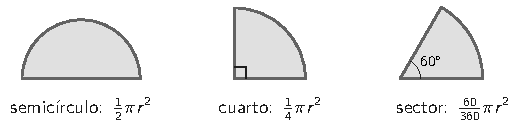
\includegraphics[width=0.5\linewidth]{geo_ci_sectores}\end{center}
\begin{ejemplo} Sector de $60°$ y radio 6: $\frac{60}{360} = \frac{1}{6}$, así que $A = \frac{1}{6} \cdot 36\pi = 6\pi$ y el arco mide $\frac{1}{6} \cdot 12\pi = 2\pi$. Semicírculo: la mitad; cuarto de círculo: la cuarta parte.\end{ejemplo}
\begin{ojo}[No olvides los lados rectos] El borde de un semicírculo es la mitad de la circunferencia \textbf{más el diámetro}: con $r = 5$, $P = 5\pi + 10$. El de un sector incluye los dos radios.\end{ojo}

\subsection{Regiones sombreadas y coronas}
\geolado[0.36]{geo_ci_sombra}{Igual que con los polígonos: área grande menos área en blanco. Un círculo que toca los cuatro lados de un cuadrado de 10 cm tiene radio 5 cm, y lo sombreado mide $100 - 25\pi \approx 21{,}5$ cm$^2$.

La \textbf{corona circular} es el anillo entre dos circunferencias de igual centro y radios $R$ y $r$: \[A = \pi R^2 - \pi r^2 = \pi(R^2 - r^2).\]}
\begin{ojo}[Corona: resta áreas, no radios] Con $R = 5$ y $r = 3$: $\pi(25 - 9) = 16\pi$. En cambio, $\pi(5 - 3)^2 = 4\pi$ está mal.\end{ojo}
\gatotip[\gatonegro]{Cuatro cuartos de círculo iguales forman un círculo completo, y dos semicircunferencias iguales, una circunferencia. ¡Junta los pedazos antes de calcular!}

\begin{elejemplo}{Tipo PAES}
\geolado[0.22]{geo_ci_ej}{En cada esquina de un cuadrado de 8 cm de lado se dibujó un cuarto de círculo con centro en el vértice y radio 4 cm, como se muestra en la figura.

¿Cuál es el área de la región sombreada?}
\alts{$(64 - 4\pi)$ cm$^2$}{$16\pi$ cm$^2$}{$(64 - 16\pi)$ cm$^2$}{$(64 - 8\pi)$ cm$^2$}
\solucion{Lo sombreado es el cuadrado menos los cuatro cuartos de círculo. El cuadrado mide $8 \cdot 8 = 64$ cm$^2$. Los cuatro cuartos, del mismo radio, forman un círculo completo de radio 4: $\pi \cdot 4^2 = 16\pi$ cm$^2$. Queda $(64 - 16\pi)$ cm$^2$.

\textit{Comprobación}: con $\pi \approx 3{,}14$, $16\pi \approx 50{,}24$ y lo sombreado mide unos 13,8 cm$^2$: positivo y menor que lo blanco \checkmark.

\textit{¿Por qué no las otras?} $(64 - 4\pi)$ resta un solo cuarto de círculo. $16\pi$ es la parte en blanco. $(64 - 8\pi)$ usa el perímetro de la circunferencia de radio 4 en vez de su área.}{C}
\end{elejemplo}
\motivacion{Los decimales de $\pi$ no se terminan nunca, y tus ganas tampoco. ¡Una vuelta completa más al temario!}

%% =====================================================================
\section{Área de superficie de cubos, paralelepípedos y cilindros}
\subsection{Los cuerpos y sus partes}
Un \textbf{paralelepípedo} (prisma recto de base rectangular) es una caja: 6 caras rectangulares, iguales de a pares. Un \textbf{cubo} tiene todas sus aristas iguales y sus 6 caras son cuadrados. Ambos tienen \textbf{6 caras, 12 aristas y 8 vértices}. Un \textbf{cilindro} tiene dos bases circulares iguales y una cara lateral curva, como una lata.
\begin{center}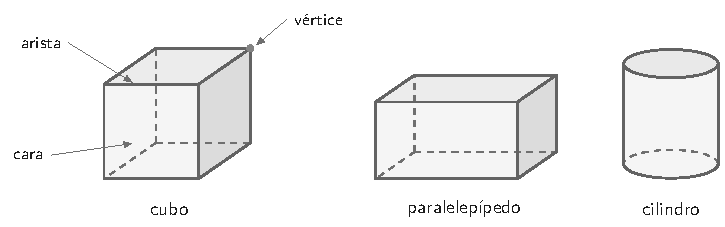
\includegraphics[width=0.62\linewidth]{geo_ac_cuerpos}\end{center}
Las líneas punteadas son aristas ocultas, que quedan detrás.

\subsection{Redes: el cuerpo desarmado}
\geolado[0.38]{geo_ac_redes}{Si desarmas una caja y la estiras sobre la mesa, obtienes su \textbf{red} o desarrollo plano. El \textbf{área de la superficie} del cuerpo es el área de su red: 6 cuadrados iguales en el cubo y 3 pares de rectángulos en el paralelepípedo.

Sirven como red de cubo la cruz y las de forma ``1--4--1''. No sirven un bloque de $2 \times 3$ ni una fila de 4 con dos cuadrados del mismo lado.}
\begin{ojo}[Truco] En una fila de 4 cuadrados, esos 4 son las paredes de alrededor; los otros dos deben ser tapa y fondo, uno a cada lado de la fila.\end{ojo}

\subsection{Área del cubo y del paralelepípedo}
\begin{clave}[Área total] Cubo de arista $a$: $6a^2$. \qquad Paralelepípedo de aristas $a$, $b$, $c$: $2(ab + bc + ac)$.\end{clave}
\begin{ejemplo} Cubo de arista 4 cm: $6 \cdot 16 = 96$ cm$^2$. Al revés, un cubo de 150 cm$^2$ tiene caras de $150 \div 6 = 25$ cm$^2$ y arista $\sqrt{25} = 5$ cm. Caja de 8, 5 y 3 cm: $2(40 + 24 + 15) = 158$ cm$^2$.\end{ejemplo}
Si el cuerpo no tiene tapa, o no se pinta la base, se resta esa cara: el cubo sin tapa tiene $5a^2$.
\begin{ojo}[No confundas con el volumen] El área total del cubo es $6a^2$ (cm$^2$); el volumen es $a^3$ (cm$^3$). Y no olvides el ``por 2'': cada tipo de cara aparece dos veces.\end{ojo}

\subsection{Área del cilindro}
\geolado[0.42]{geo_ac_red_cil}{Al abrir un cilindro, la cara lateral es un \textbf{rectángulo}: su largo es el perímetro de la base, $2\pi r$, y su ancho es la altura $h$. La etiqueta de una lata es justamente el área lateral.}
\begin{clave}[Cilindro] Lateral: $2\pi r h$ \qquad Bases: $2\pi r^2$ \qquad Total: $2\pi r h + 2\pi r^2$\end{clave}
\begin{ejemplo} Lata de radio 3 cm y altura 10 cm: lateral $60\pi$, bases $18\pi$, total $78\pi \approx 244{,}9$ cm$^2$.\end{ejemplo}
\begin{ojo}[Con diámetro] El lateral es $\pi d h$. Si pones el diámetro en lugar del radio en $2\pi r h$, el resultado sale al doble.\end{ojo}
\begin{center}\small
\begin{tabular}{lll}\toprule
Cuerpo & Área lateral & Área total\\\midrule
Cubo de arista $a$ & $4a^2$ & $6a^2$\\
Paralelepípedo $a \times b \times c$ (alto $c$) & $2(a + b)\,c$ & $2(ab + bc + ac)$\\
Cilindro de radio $r$ y altura $h$ & $2\pi r h$ & $2\pi r h + 2\pi r^2$\\\bottomrule
\end{tabular}\end{center}
\gatotip[\gatolila]{Antes de sumar, haz la lista de caras que se cuentan: ``sin tapa'', ``sin la base'', ``solo las paredes''. Y si pegas dos cuerpos, se pierden las \textbf{dos} caras que se tocan.}

\begin{elejemplo}{PAES Invierno 2026, adaptada}
\geolado[0.24]{geo_ac_mueble}{Un carpintero restaurará el siguiente mueble con forma de prisma recto de base rectangular, de 90 cm de ancho, 50 cm de fondo y 200 cm de alto.

Para la restauración, debe pintar el exterior de la estructura, sin incluir la base inferior.

¿Cuál es la medida de la superficie por pintar?}
\alts{32.500 cm$^2$}{56.000 cm$^2$}{60.500 cm$^2$}{65.000 cm$^2$}
\solucion{Calculamos el área total y le restamos la base. Frente y espalda: $2 \cdot (90 \cdot 200) = 36.000$ cm$^2$. Costados: $2 \cdot (50 \cdot 200) = 20.000$ cm$^2$. Tapa y base: $2 \cdot (90 \cdot 50) = 9000$ cm$^2$. Total: $65.000$ cm$^2$. Sin la base inferior: $65.000 - 4500 = 60.500$ cm$^2$.

\textit{Comprobación}, sumando solo lo que se pinta: $36.000 + 20.000 + 4500 = 60.500$ \checkmark.

\textit{¿Por qué no las otras?} 32.500 cm$^2$ cuenta una sola cara de cada par. 56.000 cm$^2$ quita también la tapa, que sí se pinta. 65.000 cm$^2$ incluye la base inferior.}{C}
\end{elejemplo}
\motivacion{Desarmar un cuerpo en sus caras es la clave. Ya ves las figuras por dentro y por fuera.}

%% =====================================================================
\section{Volumen de cubos, paralelepípedos y cilindros}
\subsection{¿Qué es el volumen?}
\geolado[0.28]{geo_vo_cubitos}{El \textbf{volumen} mide cuánto espacio ocupa un cuerpo: cuántos cubitos de $1 \times 1 \times 1$ caben dentro. Se mide en unidades cúbicas: cm$^3$, m$^3$.

En una caja de $4 \times 3 \times 2$ cm caben $4 \cdot 3 = 12$ cubitos en el piso y hay 2 capas: $24$ cm$^3$. Un cubo de arista $a$ tiene $V = a^3$.}
\begin{ojo}[Tres unidades distintas] Largo en cm, área en cm$^2$, volumen en cm$^3$. El volumen siempre es un producto: sumar las aristas no tiene sentido.\end{ojo}

\subsection{Paralelepípedo y cilindro}
\begin{clave}[Volumen = área de la base $\times$ altura] Cubo: $a^3$ \qquad Paralelepípedo: $a \cdot b \cdot c$ \qquad Cilindro: $\pi r^2 h$\end{clave}
\begin{ejemplo} Caja de 20, 5 y 30 cm: $3000$ cm$^3$; si se hace un 10~\% más alta, la altura pasa a 33 cm y el volumen a $3300$ cm$^3$, también un 10~\% más. Lata de radio 3 cm y altura 10 cm: $V = \pi \cdot 9 \cdot 10 = 90\pi \approx 282{,}6$ cm$^3$. Al revés: con $V = 600$, largo 10 y ancho 6, la altura es $600 \div 60 = 10$.\end{ejemplo}
\begin{ojo}[Errores del cilindro] Usar el diámetro como radio (el volumen sale 4 veces más grande), escribir $2\pi r h$ (área lateral) u olvidar elevar el radio al cuadrado. Si el cilindro está acostado, su ``altura'' es el largo.\end{ojo}

\subsection{Capacidad: litros y metros cúbicos}
La \textbf{capacidad} es el volumen que cabe dentro de un recipiente. Un cubo de 10 cm de arista contiene exactamente 1 litro.
\begin{center}\small
\begin{tabular}{ll}\toprule
Volumen & Capacidad\\\midrule
1 cm$^3$ & 1 mL\\
1 dm$^3$ $=$ 1000 cm$^3$ & 1 L\\
1 m$^3$ $=$ 1000 dm$^3$ & 1000 L\\\bottomrule
\end{tabular}\end{center}
\begin{ojo}[Tres medidas, tres veces] De m a cm se multiplica por 100, pero de m$^3$ a cm$^3$ por $100 \cdot 100 \cdot 100 = 1.000.000$. Lo más seguro es pasar las medidas a la unidad que quieras \textbf{antes} de multiplicar.\end{ojo}

\subsection{Llenado, nivel del agua y caudal}
\geolado[0.38]{geo_vo_pecera}{El agua dentro de una caja forma otra caja, con la misma base y de alto el nivel del agua.
\begin{itemize}
\item \textbf{Altura que alcanza}: 6 L $= 6000$ cm$^3$ en una pecera de base $30 \times 20$ cm suben $6000 \div 600 = 10$ cm.
\item \textbf{Objeto sumergido}: si el agua sube 2 cm, su volumen es $30 \cdot 20 \cdot 2 = 1200$ cm$^3$.
\item \textbf{Caudal}: $Q = \frac{V}{t}$. Para llenar 3000 L en 10 minutos se necesitan 300 L/min.
\end{itemize}}
\begin{ojo}[La altura del agua] Si el recipiente no está lleno, usa la altura del agua, no la del recipiente.\end{ojo}

\subsection{Cambios de escala}
\geolado[0.3]{geo_vo_escala}{Si todas las aristas se multiplican por $k$, el volumen se multiplica por $k^3$ (y el área por $k^2$): al duplicar las aristas de un cubo caben $2 \cdot 2 \cdot 2 = 8$ cubos como el original.

Si cambia una sola medida, el volumen cambia en el mismo factor. En $\pi r^2 h$ el radio cuenta doble: duplicarlo multiplica el volumen por 4; duplicar radio y altura, por 8.}
\gatotip[\gatogris]{Si un metal se funde y se rehace en piezas chicas, el volumen se conserva: divide volúmenes. Y para saber cuántas cajas caben en un contenedor, cuenta cuántas entran a lo largo de cada medida y multiplica.}

\begin{elejemplo}{PAES Invierno 2027, adaptada}
\geolado[0.26]{geo_vo_estanque}{Un estanque de agua tiene forma de prisma recto de base rectangular, cuya base mide 4 m de largo y 3 m de ancho. Se debe llenar hasta 2 m de altura con agua proveniente de un ducto.

Para calcular el caudal del agua que sale de un ducto se puede usar la expresión $\frac{V}{t}$, donde $V$ es el volumen de agua que sale del ducto durante $t$ unidades de tiempo.}
¿Cuál de las siguientes expresiones corresponde al caudal de agua, en $\frac{\text{m}^3}{\text{h}}$, que debe salir del ducto para que el estanque se llene hasta 2 m de altura en 10 horas?
\alts{$\dfrac{4 \cdot 3 \cdot 2}{10}$}{$\dfrac{4 + 3 + 2}{10}$}{$\dfrac{2(4 + 3)}{10}$}{$\dfrac{2(4 \cdot 3 + 2 \cdot 4 + 2 \cdot 3)}{10}$}
\solucion{El agua forma una caja de $4 \times 3$ m de base y 2 m de alto: $V = 4 \cdot 3 \cdot 2 = 24$ m$^3$. En $t = 10$ horas, el caudal es $\dfrac{V}{t} = \dfrac{4 \cdot 3 \cdot 2}{10}$, o sea 2,4 m$^3$ por hora.

\textit{Comprobación}: en 10 horas salen $2{,}4 \cdot 10 = 24$ m$^3$ \checkmark.

\textit{¿Por qué no las otras?} $\frac{4 + 3 + 2}{10}$ suma las medidas en vez de multiplicarlas. $\frac{2(4 + 3)}{10}$ usa el perímetro de la base por la altura, que es parte del área lateral. La última usa el área total de la caja: mide superficie, no volumen.}{A}
\end{elejemplo}
\motivacion{Llenaste otro tema hasta el borde. Tu capacidad para aprender es mucho más grande que cualquier cilindro.}

%% =====================================================================
\section{Puntos y vectores en el plano}
\subsection{El plano cartesiano y los cuadrantes}
\geolado[0.34]{tra_plano_cuadrantes}{El \textbf{plano cartesiano} tiene dos rectas numéricas perpendiculares, el \textbf{eje X} (horizontal) y el \textbf{eje Y} (vertical), que se cortan en el \textbf{origen} $O = (0, 0)$. Cada punto es un \textbf{par ordenado} $(x, y)$: primero cuánto avanzas en horizontal, después cuánto subes o bajas. $C(-2, -3)$ está 2 a la izquierda y 3 hacia abajo.

\begin{center}\small
\begin{tabular}{ccc}\toprule
Cuadrante & $x$ & $y$\\\midrule
I (arriba, derecha) & $+$ & $+$\\
II (arriba, izquierda) & $-$ & $+$\\
III (abajo, izquierda) & $-$ & $-$\\
IV (abajo, derecha) & $+$ & $-$\\\bottomrule
\end{tabular}\end{center}}

\subsection{Leer coordenadas sin equivocarse}
\textbf{El orden importa}: $(2, 5)$ y $(5, 2)$ son puntos distintos. Un punto sobre el eje X tiene $y = 0$, como $(4, 0)$; uno sobre el eje Y tiene $x = 0$, como $(0, -3)$. Los puntos de los ejes no son de ningún cuadrante.
\begin{ejemplo} Si $P(a, b)$ está en el cuadrante II, entonces $a < 0$ y $b > 0$. El punto $Q(b, a)$ tiene primera coordenada positiva y segunda negativa: está en el cuadrante IV.\end{ejemplo}
\begin{ojo}[Primero la $x$] En $(x, y)$ siempre va primero lo horizontal, como en el abecedario. Y si la cuadrícula tiene escala, multiplica los cuadros por lo que vale cada uno.\end{ojo}

\subsection{¿Qué es un vector?}
Un \textbf{vector} $\vec{u} = (a, b)$ es una flecha que indica un \textbf{desplazamiento}: $(3, 2)$ es 3 a la derecha y 2 hacia arriba. Tiene \textbf{magnitud} (su largo), \textbf{dirección} (su inclinación) y \textbf{sentido} (hacia cuál lado apunta). Flechas iguales dibujadas en distintos lugares son el mismo vector.
\begin{clave}[Vector opuesto] El opuesto de $(a, b)$ es $(-a, -b)$: misma magnitud y dirección, sentido contrario.\end{clave}

\subsection{El vector entre dos puntos: final menos inicial}
\begin{clave}[Vector de $A$ a $B$] $\overrightarrow{AB} = B - A$ (final menos inicial) \qquad Magnitud de $(a, b)$: $\sqrt{a^2 + b^2}$\end{clave}
\geolado[0.27]{tra_vector_ab}{Con $A(1, 2)$ y $B(5, -1)$: $\overrightarrow{AB} = (5 - 1, -1 - 2) = (4, -3)$: 4 a la derecha y 3 hacia abajo. Su magnitud es $\sqrt{16 + 9} = 5$.


\textit{Comprobación}: $A + (4, -3) = (5, -1) = B$ \checkmark.}
\begin{ojo}[Al revés cambia el signo] $\overrightarrow{BA} = A - B = (-4, 3)$, el opuesto de $\overrightarrow{AB}$. Y la magnitud no es la suma: $|(6, 8)| = \sqrt{100} = 10$, no 14.\end{ojo}

\subsection{Sumar vectores y multiplicarlos por un número}
\geolado[0.27]{tra_suma_vectores}{Se opera coordenada con coordenada: $(a, b) + (c, d) = (a + c, b + d)$ y $k(a, b) = (ka, kb)$.

Con $\vec{u} = (4, 1)$ y $\vec{v} = (1, 3)$: $\vec{u} + \vec{v} = (5, 4)$, $\vec{u} - \vec{v} = (3, -2)$ y $2\vec{u} = (8, 2)$. En el dibujo, la suma es hacer un desplazamiento y después el otro. Multiplicar por un número negativo da vuelta el sentido.}
\begin{ojo}[No se multiplican coordenadas] $(4, 1) + (1, 3)$ no es $(4 \cdot 1, 1 \cdot 3)$.\end{ojo}

\subsection{Trasladar un punto con un vector}
\begin{clave}[Traslación de un punto] $P' = P + \vec{v}$ \qquad y al revés \qquad $P = P' - \vec{v}$\end{clave}
\begin{ejemplo} $P(-3, 4)$ y $\vec{v} = (5, -6)$: $P' = (-3 + 5, 4 - 6) = (2, -2)$. Si $P'(1, 1)$ y $\vec{v} = (4, -2)$, entonces $P = (1 - 4, 1 - (-2)) = (-3, 3)$.\end{ejemplo}
\textbf{Dos traslaciones seguidas} equivalen a una sola con la suma de los vectores: $(2, 1)$ y luego $(3, -4)$ es lo mismo que $(5, -3)$. Con el norte hacia arriba, el este es $x$ positivo, el oeste $x$ negativo, el norte $y$ positivo y el sur $y$ negativo: ``3 km al oeste y 2 km al norte'' es $(-3, 2)$.
\gatotip[\gatonaranjo]{Comprueba siempre: el punto original más el vector debe darte la imagen. Y restar un negativo es sumar: $1 - (-2) = 3$.}
\gatotip[\gatoatigrado]{En un paralelogramo $ABCD$, el vector de $A$ a $D$ es igual al de $B$ a $C$: $D = A + (C - B)$.}

\begin{elejemplo}{PAES Invierno 2026, adaptada}
Un barco que inicia un recorrido realiza los siguientes movimientos, en este orden: 4 kilómetros al oeste, 6 kilómetros al norte, 7 kilómetros al este, 9 kilómetros al sur y 5 kilómetros al oeste.

¿Cuál es la ubicación final del barco con respecto a su ubicación inicial?
\alts{2 kilómetros al este y 3 kilómetros al norte}{16 kilómetros al oeste y 15 kilómetros al sur}{2 kilómetros al oeste y 3 kilómetros al sur}{3 kilómetros al oeste y 2 kilómetros al sur}
\solucion{Cada movimiento es un vector, con este y norte positivos: $(-4, 0)$, $(0, 6)$, $(7, 0)$, $(0, -9)$ y $(-5, 0)$. El desplazamiento total es la suma. Horizontal: $-4 + 7 - 5 = -2$, o sea 2 km al oeste. Vertical: $6 - 9 = -3$, o sea 3 km al sur. El barco termina en $(-2, -3)$: 2 km al oeste y 3 km al sur.
\begin{center}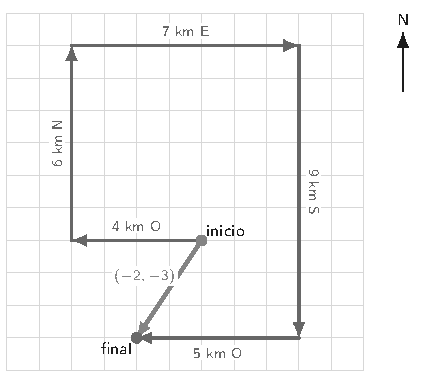
\includegraphics[width=0.3\linewidth]{tra_barco}\end{center}
\textit{Comprobación}: en la cuadrícula, la flecha que une el inicio con el final avanza 2 cuadros a la izquierda y baja 3 \checkmark.

\textit{¿Por qué no las otras?} ``2 al este y 3 al norte'' tiene los sentidos al revés. ``16 al oeste y 15 al sur'' suma todos los kilómetros sin fijarse en el sentido. ``3 al oeste y 2 al sur'' intercambia lo horizontal con lo vertical.}{C}
\end{elejemplo}
\motivacion{Ya te mueves en el plano con coordenadas y vectores. Tu vector apunta directo a la meta.}

%% =====================================================================
\section{Traslación y reflexión}
\subsection{Transformaciones isométricas}
Una \textbf{transformación isométrica} mueve una figura sin deformarla: la imagen tiene la misma forma y el mismo tamaño. Hay tres: \textbf{traslación} (desliza según un vector), \textbf{reflexión} (refleja como un espejo respecto de una recta o de un punto) y \textbf{rotación} (gira en torno a un punto). La imagen del punto $A$ se escribe $A'$.
\begin{center}\small
\begin{tabular}{lccc}\toprule
¿Se conserva? & Traslación & Reflexión & Rotación\\\midrule
Lados, ángulos, perímetro y área & sí & sí & sí\\
Orientación (sentido de recorrido de los vértices) & sí & \textbf{no}, se invierte & sí\\\bottomrule
\end{tabular}\end{center}

\subsection{Traslación de una figura}
\begin{clave}[Traslación según $(a, b)$] $(x, y) \to (x + a, y + b)$\end{clave}
\geolado[0.36]{tra_tras_triangulo}{Se traslada \textbf{cada vértice} con el mismo vector y se unen las imágenes.

Con $A(-5, 1)$, $B(-2, 1)$, $C(-4, 4)$ y $\vec{v} = (6, -3)$: $A'(1, -2)$, $B'(4, -2)$ y $C'(2, 1)$. La figura no gira ni se da vuelta. Si conoces un vértice y su imagen, el vector es imagen menos original.}

\subsection{Reflexión respecto de los ejes}
\geolado[0.3]{tra_refl_ejes}{En una reflexión, cada punto y su imagen quedan a la misma distancia del eje, uno a cada lado, en una línea perpendicular al eje.

\textbf{Respecto del eje X} la $x$ queda igual y la $y$ cambia de signo: $(x, y) \to (x, -y)$; $(3, 5) \to (3, -5)$.

\textbf{Respecto del eje Y} la $y$ queda igual y la $x$ cambia de signo: $(x, y) \to (-x, y)$; $(3, 5) \to (-3, 5)$.

La letra F de la figura queda ``al revés'', como en un espejo.}
\begin{ojo}[Para no confundirte] Cambia la coordenada que \textbf{no} lleva el nombre del eje. Reflejar respecto del eje X manda la figura hacia abajo.\end{ojo}

\subsection{\texorpdfstring{Reflexión respecto de las rectas $x = a$ e $y = b$}{Reflexión respecto de las rectas x = a e y = b}}
\geolado[0.34]{tra_refl_recta}{Cuenta la distancia del punto a la recta y pasa la misma distancia al otro lado. $B(1, 1)$ respecto de $x = 3$: de 1 a 3 hay 2 unidades; $3 + 2 = 5$ y la altura no cambia, $B' = (5, 1)$.}
\begin{clave}[Fórmulas] Respecto de $x = a$: $(x, y) \to (2a - x,\ y)$. \qquad Respecto de $y = b$: $(x, y) \to (x,\ 2b - y)$.\end{clave}
El eje queda justo \textbf{al medio} entre un punto y su imagen: el promedio de 1 y 5 es 3. Así se encuentra el eje si te dan un punto y su imagen.

\subsection{\texorpdfstring{Reflexión respecto de $y = x$ y respecto del origen}{Reflexión respecto de y = x y respecto del origen}}
\geolado[0.32]{tra_refl_yx}{\textbf{Respecto de la recta $y = x$} las coordenadas se intercambian: $(4, 1) \to (1, 4)$ y $(-2, 3) \to (3, -2)$.

\textbf{Respecto del origen} las dos coordenadas cambian de signo: $(4, 1) \to (-4, -1)$. Es lo mismo que reflejar respecto del eje X y luego del eje Y, y que girar $180^\circ$ en torno al origen.}
\begin{center}\small
\begin{tabular}{cccccc}\toprule
eje X & eje Y & recta $x = a$ & recta $y = b$ & recta $y = x$ & origen\\\midrule
$(x, -y)$ & $(-x, y)$ & $(2a - x, y)$ & $(x, 2b - y)$ & $(y, x)$ & $(-x, -y)$\\\bottomrule
\end{tabular}\end{center}
\begin{ojo}[Con $y = x$ no cambian los signos] Solo se intercambian: $(4, -1) \to (-1, 4)$.\end{ojo}

\subsection{Dos transformaciones seguidas}
Se hace la primera y a su resultado se le aplica la segunda. \textbf{El orden importa}.
\begin{ejemplo} $P(2, 3)$: reflexión respecto del eje X, $(2, -3)$, y luego traslación según $(1, 4)$, $(3, 1)$. En el otro orden da $(3, -7)$. Si la regla es $(x + 1, 4 - y)$, eso es reflejar respecto del eje X y trasladar según $(1, 4)$: la imagen de $(5, -2)$ es $(6, 6)$.\end{ejemplo}
\begin{clave}[Dos reflexiones] Respecto del mismo eje dos veces: el punto vuelve. Respecto de dos rectas paralelas: una traslación del doble de la distancia entre ellas. Respecto del eje X y luego del eje Y: la reflexión respecto del origen.\end{clave}
\gatotip[\gatoblanco]{Doblar papel es reflejar: si perforas una hoja doblada, al abrirla la perforación aparece reflejada respecto de la línea del doblez. Para deshacer dos transformaciones, deshazlas en orden inverso.}

\begin{elejemplo}{PAES Invierno 2026, adaptada}
A una figura se le aplica una reflexión y luego una traslación. La imagen del vértice $(x, y)$ es $(x - 3, 4 - y)$. A otra figura se le aplican las mismas transformaciones isométricas y en el mismo orden.

Si $(-2, -5)$ es un vértice de esta figura, ¿cuáles son las coordenadas de la imagen de este vértice?
\alts{$(-5, -1)$}{$(5, 9)$}{$(-5, 9)$}{$(-5, -9)$}
\solucion{Basta reemplazar $x = -2$ e $y = -5$ en la regla: $x - 3 = -2 - 3 = -5$ y $4 - y = 4 - (-5) = 9$. La imagen es $(-5, 9)$.

\textit{Comprobación} por pasos: la regla es una reflexión respecto del eje X seguida de una traslación según $(-3, 4)$; $(-2, -5) \to (-2, 5) \to (-5, 9)$ \checkmark.

\textit{¿Por qué no las otras?} $(-5, -1)$ calcula $4 + y$. $(5, 9)$ cambia el signo de la $x$. $(-5, -9)$ se equivoca con el menos: escribe $4 - (-5)$ como $-(4 + 5)$.}{C}
\end{elejemplo}
\motivacion{Trasladar y reflejar no cambian la figura, solo su lugar. Tú sí estás cambiando: cada tema te hace más fuerte.}

%% =====================================================================
\section{Rotación}
\subsection{¿Qué es una rotación?}
Una \textbf{rotación} gira una figura en torno a un punto fijo, el \textbf{centro de rotación}. Se describe con tres datos: el \textbf{centro} (casi siempre el origen), el \textbf{ángulo} (en la PAES, $90^\circ$, $180^\circ$ o $270^\circ$) y el \textbf{sentido}: \textbf{horario}, como los punteros del reloj, o \textbf{antihorario}, al revés. Cada punto se mantiene a la misma distancia del centro, así que la figura no cambia de tamaño ni se da vuelta.

\subsection{Las reglas de 90°, 180° y 270°}
\geolado[0.34]{tra_rot_tabla}{\begin{center}\small
\begin{tabular}{lcc}\toprule
Rotación en torno al origen & Regla & $P(4, 2)$\\\midrule
$90^\circ$ antihorario & $(-y, x)$ & $(-2, 4)$\\
$180^\circ$ (cualquier sentido) & $(-x, -y)$ & $(-4, -2)$\\
$270^\circ$ antihorario $= 90^\circ$ horario & $(y, -x)$ & $(2, -4)$\\
$360^\circ$ & $(x, y)$ & $(4, 2)$\\\bottomrule
\end{tabular}\end{center}
$270^\circ$ en un sentido es lo mismo que $90^\circ$ en el otro. $180^\circ$ da igual en un sentido o en el otro, y equivale a la reflexión respecto del centro.}
\begin{ejemplo} $90^\circ$ horario a $P(-2, 5)$: $(y, -x) = (5, 2)$. $90^\circ$ antihorario a $(4, -1)$: $(-y, x) = (1, 4)$, porque $-(-1) = 1$.\end{ejemplo}

\subsection{Trucos para no girar al revés}
\begin{clave}[Los cuadrantes] Con $90^\circ$ antihorario, cada punto avanza un cuadrante: I $\to$ II $\to$ III $\to$ IV $\to$ I. Con $90^\circ$ horario retrocede uno. Con $180^\circ$ va al cuadrante opuesto.\end{clave}
También sirve girar la hoja un cuarto de vuelta, o probar con $(1, 0)$: con $90^\circ$ antihorario debe quedar arriba, en $(0, 1)$. Varias rotaciones con el mismo centro se suman: tres de $90^\circ$ antihorario son $270^\circ$, o sea $90^\circ$ horario; cuatro devuelven la figura. Para deshacer una rotación, gira el mismo ángulo en sentido contrario.
\gatotip[\gatolila]{Los punteros del reloj giran en sentido horario, y el minutero avanza $360^\circ \div 60 = 6^\circ$ por minuto: en 20 minutos gira $120^\circ$.}

\subsection{Rotar en torno a otro punto}
\begin{clave}[Centro $C$] Mira el punto desde el centro, gíralo y vuelve: 1. resta el centro, $P - C$; 2. aplica la regla; 3. suma el centro.\end{clave}
\geolado[0.27]{tra_rot_centro}{$P(5, 2)$ en $90^\circ$ antihorario en torno a $C(2, 1)$: $P - C = (3, 1) \to (-1, 3)$, y sumando $C$, $P' = (1, 4)$.}
\begin{ojo}[No olvides volver] Quedarse con $(-1, 3)$ es el error más común: esa es la posición respecto de $C$. Con $180^\circ$, el centro es el punto medio entre el punto y su imagen: $P' = 2C - P$.\end{ojo}

\subsection{¿Qué transformación es?}
\geolado[0.28]{tra_rot_identificar}{Para reconocer qué transformación lleva una figura a otra:

\textbf{1. ¿Está dada vuelta?} Si se ve como en un espejo, es una \textbf{reflexión}.

\textbf{2. Si no, ¿está girada?} Si apunta en otra dirección, es una \textbf{rotación}; si apunta igual y solo cambió de lugar, es una \textbf{traslación}.

Después confirma aplicando la regla a un vértice. La F girada en $180^\circ$ queda cabeza abajo, pero se puede leer girando la hoja; la reflejada no.}
\gatotip[\gatonegro]{Para seguir una flecha, usa ángulos: este $0^\circ$, noreste $45^\circ$, norte $90^\circ$, sur $270^\circ$. Rotar en sentido antihorario suma grados, y una traslación nunca cambia hacia dónde apunta.}

\begin{elejemplo}{PAES Invierno 2027, adaptada}
\geolado[0.32]{tra_rot_proteina}{En el gráfico se representa una simulación bidimensional de una proteína con su grupo metilo, localizado en el punto $P(5, 3)$, con el objetivo de estudiar su desplazamiento. Dicha proteína con su grupo metilo es sometida a una rotación de $90^\circ$ en sentido antihorario con respecto al origen del sistema de coordenadas cartesianas.

¿Cuáles son las coordenadas del grupo metilo después de la rotación?}
\alts{$(3, -5)$}{$(-3, 5)$}{$(-5, -3)$}{$(5, -3)$}
\solucion{La regla de $90^\circ$ antihorario en torno al origen es $(x, y) \to (-y, x)$. Con $x = 5$ e $y = 3$ queda $(-3, 5)$.

\textit{Comprobación}: $P$ estaba en el cuadrante I y la imagen está en el II, como corresponde; además la distancia al origen se mantiene, $\sqrt{25 + 9} = \sqrt{9 + 25} = \sqrt{34}$ \checkmark.

\textit{¿Por qué no las otras?} $(3, -5)$ gira $90^\circ$ en sentido horario. $(-5, -3)$ gira $180^\circ$. $(5, -3)$ refleja respecto del eje X.}{B}
\end{elejemplo}
\motivacion{Girar en 90 o 180 grados ya no es un misterio. Y si algo sale mal, das la vuelta y lo intentas otra vez.}

%% =====================================================================
\section{Semejanza y escalas}
\subsection{Figuras semejantes}
Dos figuras son \textbf{semejantes} ($\sim$) si tienen la misma forma, aunque distinto tamaño: una es ampliación o reducción de la otra. Sus \textbf{ángulos} correspondientes son iguales y sus \textbf{lados} son \textbf{proporcionales}: todos se multiplican por el mismo número $k$, la \textbf{razón de semejanza}.
\begin{center}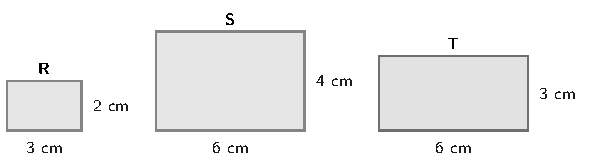
\includegraphics[width=0.52\linewidth]{sem_rectangulos}\end{center}
\begin{ejemplo} $R$ mide $3 \times 2$ y $S$ mide $6 \times 4$: $\frac{6}{3} = \frac{4}{2} = 2$, son semejantes con $k = 2$. $T$ mide $6 \times 3$: $\frac{6}{3} = 2$, pero $\frac{3}{2} = 1{,}5$; no es semejante a $R$.\end{ejemplo}
\begin{ojo}[Proporcional no es sumar lo mismo] Sumarle 3 a cada lado de $3 \times 2$ da $6 \times 5$, que no es semejante. En la semejanza se \textbf{multiplica}.\end{ojo}

\subsection{Lados homólogos y razón de semejanza}
Los \textbf{lados homólogos} son los que se corresponden. Si $\triangle ABC \sim \triangle DEF$, el orden de las letras lo dice: $AB$ con $DE$, $BC$ con $EF$ y $AC$ con $DF$.
\begin{ejemplo} $\triangle ABC \sim \triangle DEF$ con $AB = 3$, $BC = 4$, $AC = 5$, $DE = 6$ y $DF = 10$. La razón es $k = \frac{DE}{AB} = 2$ (y $\frac{DF}{AC} = 2$ lo confirma), así que $EF = 2 \cdot 4 = 8$. Con proporción: $\frac{x}{4} = \frac{6}{3}$, $3x = 24$, $x = 8$.\end{ejemplo}

\subsection{Triángulos semejantes: basta con dos ángulos}
\geolado[0.3]{sem_encajados}{Dos triángulos con \textbf{dos ángulos iguales} son semejantes (criterio AA); el tercero también es igual, porque suman $180^\circ$. También lo son si sus tres lados son proporcionales (LLL) o si dos lados son proporcionales y el ángulo entre ellos es igual (LAL).

Si en $ABC$ se traza $DE$ paralelo a $BC$, el triángulo $ADE$ es semejante a $ABC$. Con $AD = 2$, $DB = 4$ y $DE = 3$: $AB = 6$, $k = \frac{6}{2} = 3$ y $BC = 3 \cdot 3 = 9$.}
\begin{ojo}[El error clásico] El homólogo de $AB$ (lado completo del grande) es $AD$ (lado completo del chico), no el pedazo $DB$.\end{ojo}

\subsection{Sombras, postes y alturas}
\geolado[0.4]{sem_sombras}{A la misma hora, los rayos del sol llegan paralelos: cada objeto vertical, su sombra y el rayo forman triángulos rectángulos semejantes. La razón altura\,:\,sombra es la misma para todos.

Un poste de 4 m da 6 m de sombra. Una persona de 1,6 m da $\frac{1{,}6}{x} = \frac{4}{6}$, o sea $4x = 9{,}6$ y $x = 2{,}4$ m.}
\begin{ojo}[Ordena antes de calcular] Alturas arriba y sombras abajo en las dos fracciones; si mezclas, el resultado sale al revés.\end{ojo}
\gatotip[\gatogris]{Espejos en el suelo, rampas con soportes y ríos que no se pueden cruzar esconden lo mismo: dos triángulos semejantes. Empareja los lados homólogos y escribe la misma razón en ambos.}

\subsection{Planos, mapas y maquetas a escala}
Una \textbf{escala $1 : n$} significa que 1 cm del dibujo representa $n$ cm de la realidad. Del dibujo a la realidad se multiplica por $n$; de la realidad al dibujo se divide.
\begin{ejemplo} Mapa 1\,:\,50.000 con 6 cm entre dos pueblos: $6 \cdot 50.000 = 300.000$ cm $= 3000$ m $= 3$ km. Edificio de 45 m en maqueta 1\,:\,300: $\frac{4500}{300} = 15$ cm. Si 2 cm del mapa son 200 m $= 20.000$ cm, 1 cm son 10.000 cm: escala 1\,:\,10.000.\end{ejemplo}
\begin{ojo}[Mismas unidades] La escala compara centímetros con centímetros: 1 m $= 100$ cm, 1 km $= 100.000$ cm y 1 m$^2$ $= 10.000$ cm$^2$. En una escala gráfica, como ``2 cm $=$ 1 km'', cuenta cuántas veces cabe la barra.\end{ojo}

\subsection{\texorpdfstring{Perímetro por $k$, área por $k^2$}{Perímetro por k, área por k al cuadrado}}
\geolado[0.3]{sem_areas}{Si una figura se amplía con razón $k$, cada \textbf{longitud} (lados, perímetro, alturas) se multiplica por $k$ y el \textbf{área} por $k^2$: al duplicar el lado de un cuadrado caben $2 \cdot 2 = 4$ cuadrados como el original.}
\begin{ejemplo} Triángulo de perímetro 10 cm y área 4 cm$^2$, ampliado con $k = 3$: perímetro 30 cm y área $4 \cdot 9 = 36$ cm$^2$. Al revés: si las áreas de dos cuadrados son 9 y 36, $k^2 = 4$ y $k = 2$. En un plano 1\,:\,100 las áreas se multiplican por $100^2 = 10.000$.\end{ejemplo}
\gatotip[\gatoatigrado]{En un plano a escala, lo más seguro es pasar primero cada lado a la realidad y después calcular el área. Y revisa al final: lo grande debe quedar grande y lo chico, chico.}

\begin{elejemplo}{PAES Invierno 2027, adaptada}
\geolado[0.3]{sem_mapa_ruta}{Martina debe ir de su casa al colegio y para esto revisa un mapa. En la figura se presenta el mapa y la medida, en el mapa, del recorrido que debe hacer. Se sabe que 3 cm en el mapa equivalen a 150 m de distancia en la realidad.

¿Cuál es la distancia real que debe recorrer Martina?}
\alts{450 m}{650 m}{1950 m}{50 m}
\solucion{Si 3 cm son 150 m, entonces 1 cm del mapa es $\frac{150}{3} = 50$ m. El recorrido mide 13 cm en el mapa: $13 \cdot 50 = 650$ m.

\textit{Comprobación} con una proporción: $\frac{3}{150} = \frac{13}{x}$, así que $3x = 1950$ y $x = 650$ \checkmark.

\textit{¿Por qué no las otras?} 450 m multiplica 150 m por 3. 1950 m supone que cada centímetro vale 150 m. 50 m es lo que vale un solo centímetro.}{B}
\end{elejemplo}
\motivacion{Misma forma, distinto tamaño: en el mapa tus metas se ven chicas, pero a escala real son enormes. Cerraste Geometría: ¡bravo!}

